\documentclass[a4paper, 10pt, twoside]{article}

\usepackage[top=1in, bottom=1in, left=1in, right=1in]{geometry}
\usepackage[utf8]{inputenc}
\usepackage[spanish, es-ucroman, es-noquoting]{babel}
\usepackage{setspace}
\usepackage{fancyhdr}
\usepackage{lastpage}
\usepackage{amsmath}
\usepackage{amsfonts}
\usepackage{amsthm}
\usepackage{verbatim}
\usepackage{fancyvrb}
\usepackage{graphicx}
\usepackage{float}
\usepackage{enumitem} % Provee macro \setlist
\usepackage{tabularx}
\usepackage{multirow}
\usepackage{hyperref}
\usepackage{lscape}
\usepackage{xspace}
\usepackage{qtree}
\usepackage[toc, page]{appendix}


%%%%%%%%%% Constantes - Inicio %%%%%%%%%%
\newcommand{\titulo}{Trabajo Práctico 2}
\newcommand{\materia}{Ingeniería de Software II}
\newcommand{\integrantes}{Izcovich · Lovisolo · Petaccio · Vita}
\newcommand{\cuatrimestre}{Primer Cuatrimestre de 2015}
%%%%%%%%%% Constantes - Fin %%%%%%%%%%


%%%%%%%%%% Configuración de Fancyhdr - Inicio %%%%%%%%%%
\pagestyle{fancy}
\thispagestyle{fancy}
\lhead{\titulo\ · \materia}
\rhead{\integrantes}
\renewcommand{\footrulewidth}{0.4pt}
\cfoot{\thepage /\pageref{LastPage}}

\fancypagestyle{caratula} {
   \fancyhf{}
   \cfoot{\thepage /\pageref{LastPage}}
   \renewcommand{\headrulewidth}{0pt}
   \renewcommand{\footrulewidth}{0pt}
}
%%%%%%%%%% Configuración de Fancyhdr - Fin %%%%%%%%%%


%%%%%%%%%% Miscelánea - Inicio %%%%%%%%%%
% Evita que el documento se estire verticalmente para ocupar el espacio vacío
% en cada página.
\raggedbottom

% Separación entre párrafos.
\setlength{\parskip}{0.5em}

% Separación entre elementos de listas.
\setlist{itemsep=0.5em}

% Asigna la traducción de la palabra 'Appendices'.
\renewcommand{\appendixtocname}{Apéndices}
\renewcommand{\appendixpagename}{Apéndices}

\newcommand{\diagrama}[1]{
  \begin{center}
    \includegraphics[width=16cm]{#1}
  \end{center}
}

\newcommand{\diagramadeancho}[2]{
  \begin{center}
    \includegraphics[width=#1]{#2}
  \end{center}
}

\newcommand{\riesgo}[7]{
  \underline{Riesgo {#1}:}
  \begin{itemize}   
    \item \textbf{Descripción:} {#2}
    \item \textbf{Probablidad:} {#3}
    \item \textbf{Impacto:} {#4}
    \item \textbf{Exposición:} {#5}
    \item \textbf{Mitigación:} {#6}
    \item \textbf{Plan de contingencia:} {#7}
  \end{itemize}
}

\newcommand{\escenario}[7] {
  \textit{{#1}}
  \begin{itemize}
    \item \textbf{Fuente:} {#2}
    \item \textbf{Estímulo:} {#3}
    \item \textbf{Entorno:} {#4}
    \item \textbf{Artefacto:} {#5}
    \item \textbf{Respuesta:} {#6}
    \item \textbf{Medición:} {#7}
  \end{itemize}
}

%%%%%%%%%% Miscelánea - Fin %%%%%%%%%%

\begin{document}


%%%%%%%%%%%%%%%%%%%%%%%%%%%%%%%%%%%%%%%%%%%%%%%%%%%%%%%%%%%%%%%%%%%%%%%%%%%%%%%
%% Carátula                                                                  %%
%%%%%%%%%%%%%%%%%%%%%%%%%%%%%%%%%%%%%%%%%%%%%%%%%%%%%%%%%%%%%%%%%%%%%%%%%%%%%%%


\thispagestyle{caratula}

\begin{center}


\includegraphics[height=2cm]{DC.png} 
\hfill

\includegraphics[height=2cm]{UBA.jpg} 

\vspace{2cm}

Departamento de Computación,\\
Facultad de Ciencias Exactas y Naturales,\\
Universidad de Buenos Aires

\vspace{4cm}

\begin{Huge}
\titulo
\end{Huge}

\vspace{0.5cm}

\begin{Large}
\materia
\end{Large}

\vspace{1cm}

\cuatrimestre

\vspace{4cm}

\begin{tabular}{|c|c|c|}
\hline
Apellido y Nombre & LU & E-mail\\
\hline
Izcovich, Sabrina      & 550/11 & sizcovich@gmail.com\\
Lovisolo, Leandro      & 645/11 & leandro@leandro.me\\
Petaccio, Lautaro José & 443/11 & lausuper@gmail.com\\
Vita, Sebastián        & 149/11 & sebastian\_vita@yahoo.com.ar\\
\hline
\end{tabular}

\end{center}

\newpage

\tableofcontents

\newpage


%%%%%%%%%%%%%%%%%%%%%%%%%%%%%%%%%%%%%%%%%%%%%%%%%%%%%%%%%%%%%%%%%%%%%%%%%%%%%%%
%% Introducción                                                              %%
%%%%%%%%%%%%%%%%%%%%%%%%%%%%%%%%%%%%%%%%%%%%%%%%%%%%%%%%%%%%%%%%%%%%%%%%%%%%%%%

\section{Introducción}

En el presente trabajo se aborda la extensión del diseño presentado en el TP1, debiendo ahora plantear un sistema de mensajes de muchas campañas a nivel nacional tanto para servicios públicos como privados. Dada esta nueva situación, aparecen varios stakeholders que, por su colaboración en el proyecto proveyendo servicios, o por su intención de consumo, imponen distintos requerimientos que sumados a los técnicos desembocan en la contemplación de diversos riesgos y atributos de calidad.
Aquí se presenta una planificación de las fases de elaboración, construcción y transición de la metodología UP, asumiendo que la fase inception ya se ha desarrollado. En esta primera etapa se presentan las ideas para la formulación del proyecto Big Tiza, se establecen los requerimientos y recursos disponibles, y se lleva a cabo el QAW del cual se desprendieron algunos atributos de calidad esperados en el producto final. Como parte de la primera iteración, se identifican los casos de uso más relevantes y en base a la recopilación de toda esta información se realiza un análisis de riesgos que se utiliza en parte para la organización de los CU en las distintas iteraciones incrementales. Además se diseña la arquitectura del sistema.

\newpage

%%%%%%%%%%%%%%%%%%%%%%%%%%%%%%%%%%%%%%%%%%%%%%%%%%%%%%%%%%%%%%%%%%%%%%%%%%%%%%%
%% Casos de uso                                                              %%
%%%%%%%%%%%%%%%%%%%%%%%%%%%%%%%%%%%%%%%%%%%%%%%%%%%%%%%%%%%%%%%%%%%%%%%%%%%%%%%

\section{Casos de uso}
Para comenzar a trabajar sobre la planificación del proyecto se identificó un conjunto de casos de uso que cubren la mayoría de las funcionalidades que se desprenden de los requerimientos obtenidos. En un principio se los agrupó, tal y como se muestra a continuación, por su funcionalidad. Posteriormente, y en base al análisis de riesgos y a la información destilada de la fase de incepción, se utilizó este refinamiento para la organización y planificación de las iteraciones de elaboración y construcción.

\begin{itemize}

\item \textbf{Comunicación}
\begin{itemize}
\item Enviando mensajes de campañas por medios seleccionados\footnote{Facebook, Twitter, Whatsapp o SMS.}.
\item Respondiendo mensaje a una pregunta.
\end{itemize}

\item \textbf{Monitoreo}
\begin{itemize}
\item Consultando estado de una campaña.
\item Visualizando el mapa de evolución de las campañas.
\end{itemize}

\item \textbf{Auditoría}
\begin{itemize}
\item Registrando cantidad de mensajes enviados por campaña.
\item Generando factura mensual para la empresa de infraestructura privada.
\end{itemize}

\item \textbf{Gestión}
\begin{itemize}
\item Ingresando los resultados de una campaña.
\item Creando, editando y eliminando grupos de destinatarios.
\item Creando una campaña desde el sector público/privado.
\item Desuscribiendo a un destinatario de una campaña.
%\item Reinscribiendo a un destinatario en una campaña de la que se desuscribió.
\item Agregando evaluación manual del resultado de las preguntas.
\item Aceptando campaña privada.
\item Creando cuestionario de campañas de evaluación de campañas.
\item Agregando nuevo usuario proveedor de contenidos.
\item Creando, editando y eliminando usuarios.
\end{itemize}

\item \textbf{Supervisión}
\begin{itemize}
\item Supervisando campañas privadas (supervisar encuestas)?
\item Pidiendo reportes de resultados de una campaña
\item Reportando información anonimizada de grupos de destinatarios.
\end{itemize}

\item \textbf{Seguridad}
\begin{itemize}
\item Autenticando usuario.
\item Guardando datos cifrados en servidores locales.
\end{itemize}
\end{itemize}

\newpage

%%%%%%%%%%%%%%%%%%%%%%%%%%%%%%%%%%%%%%%%%%%%%%%%%%%%%%%%%%%%%%%%%%%%%%%%%%%%%%%
%% Planificación                                                          %%
%%%%%%%%%%%%%%%%%%%%%%%%%%%%%%%%%%%%%%%%%%%%%%%%%%%%%%%%%%%%%%%%%%%%%%%%%%%%%%%

\section{Planificación}

\subsection{Iteraciones}
La división de los CU en las distintas iteraciones y la organización de las mismas estuvo pautada por las necesidades manifestadas por los stakeholders, el análisis de riesgo y un incremento de funcionalidad, partiendo del núcleo más importante y revistiendo la aplicación a lo largo del tiempo de lógica menos prioritaria.

\subsubsection{Fase de iniciación}
Consideramos fase de iniciación al trabajo realizado en el Primer Trabajo Práctico junto con la Arquitectura presente en este TP.

\subsubsection{Fase de elaboración}

\textbf{Primera iteración} [3 semanas]
\begin{enumerate}
\item Guardando datos cifrados en servidores locales.
\item Creando una campaña desde el sector público/privado.
\item Enviando mensajes de campañas por medios seleccionados.
\item Autenticando usuario.
\end{enumerate}

\textbf{Segunda iteración} [5 semanas]
\begin{enumerate}
\item Creando, editando y eliminando usuarios.
\item Consultando estado de una campaña.
\item Registrando cantidad de mensajes enviados por campaña.
\item Creando, editando y eliminando grupos de destinatarios.
\end{enumerate}

\textbf{Tercera iteración} [5 semanas]
\begin{enumerate}
\item Creando cuestionario de campañas de evaluación de campañas.
\item Respondiendo mensaje a una pregunta.
\item Desuscribiendo a un destinatario de una campaña.
\item Reinscribiendo a un destinatario en una campaña de la que se desuscribió.
\end{enumerate}

\textbf{Cuarta iteración} [4 semanas]
\begin{enumerate}
\item Ingresando los resultados de una campaña.
\item Pidiendo reportes de resultados de una campaña.
\item Agregando evaluación manual del resultado de las preguntas.
\end{enumerate}

\textbf{Quinta iteración} [4 semanas]
\begin{enumerate}
\item Aceptando campaña privada.
\item Reportando información anonimizada de grupos de destinatarios.
\item Generando factura mensual para el sector privado.
\item Enviando resultados de campañas a la NSA.
\end{enumerate}

\textbf{Sexta iteración} [4 semanas]
\begin{enumerate}
\item Supervisando campañas privadas (supervisar encuestas).
\item Visualizando el mapa de evolución de las campañas.
\item Agregando nuevo usuario proveedor de contenidos.
\end{enumerate}

\subsubsection{Fase de construcción}
En la fase de construcción se crea el producto. Para poder lograrlo, se van desarrollando los casos de uso de cada una de las iteraciones previamente definidas en la etapa de elaboración. Al finalizar el desarrollo de cada una de las iteraciones, se debe contar con un software funcional que responda a todas las especificaciones. Además se debe proveer de casos de prueba para poder constatar el correcto funcionamiento del programa.

\subsubsection{Fase de transición}
En esta fase, el sistema ya se encuentra funcionando en una versión $Beta$. Esto permite poder arreglar problemas que se encuentran en el funcionamiento y que no fueron detectados en la fase anterior. Por otro lado, se utiliza esta fase tanto para poder enseñarle a los usuarios como manejar el sistema, como para extender la funcionabilidad del mismo en el caso de que sea necesario.

\subsection{Alcance de casos de usos de la primera iteración}
\textbf{Guardando datos cifrados en servidores locales.}

Los datos de los usuarios deben almacenarse encriptados en los servidores locales de su región correspondiente para poder garantizar la confidencialidad de los mismos.

Llamamos datos a los registros en la base de datos que contienen información sobre los residentes de la región. Estos pueden ser datos básicos como por ejemplo (nombre, apellido, dni, número de teléfono) y datos adiciones como si es fumador, si poseen un auto, si les gusta correr, etc.

\textbf{Creando una campaña desde el sector público/privado.}

La creación de una campaña consiste en el ingreso de los datos necesarios para la creación de la misma, es decir, un conjunto de mensajes con el horario en el que deben ser enviados, un conjunto de grupos de destinatarios concernientes al objetivo de la campaña y el canal a través del que se enviarán (SMS, Facebook, etc).

\textbf{Enviando mensajes de campañas por medios seleccionados.}

Cada región tiene un sistema de envío de mensajes que periódicamente recorre las campañas asociadas a esa región y envía los mensajes de las mismas cumpliendo su fecha y hora de envío. Además, cada mensaje es enviado por los canales previamente seleccionados a través de la infraestructura propia de cada región.

\textbf{Autenticando usuario.}

Se solicita un usuario y contraseña cuando una persona intenta iniciar una sesión en el sistema para crear una campaña y consultar el estado de una campaña, entre otras. La autenticación también abarca al sector privado dónde tendran acceso sólo a acciones de su sector.

El sistema verifica que las credenciales ingresadas sean válidas, y en caso contrario deniega el acceso al mismo.

\subsection{Tareas CU Primera iteración}
A continuación se detallan las tareas diagramadas para los casos de uso incluidos en la primera iteración con su respectiva estimación de horas hombre.
\\

\begin{tabular}{lp{13cm}l}
  \hline
  CU1 & Guardando datos cifrados en servidores locales & 140h \\
  \hline
  T01 & Investigación de fuentes de información disponibles de cada usuario accesible desde el sistema & 16h \\
  T02 & Definición de campos relevantes para almacenar por usuario & 12h \\
  T03 & Diseño de la base de datos & 16h \\
  T04 & Definición de motor de búsqueda a utilizar & 8h \\
  T05 & Definición de método de encriptación & 8h \\
  T06 & Implementación de CU1 & 40h\\
  T07 & Testing de CU1 & 40h \\
  \hline
\end{tabular}

\vspace{1em}

\begin{tabular}{lp{13cm}l}
  \hline
  CU2 & Creando una campaña desde el sector público/privado & 42h \\
  \hline
  T01 & Investigar librerías y herramientas para la implementación de las campañas & 8h \\
  T02 & Diseño de la interfaz del usuario & 4h \\
  T03 & Implementación de CU2 & 15h \\
  T04 & Testing de CU2 & 15h \\
  \hline
\end{tabular}

\vspace{1em}

\begin{tabular}{lp{13cm}l}
  \hline
  CU3 &  Enviando mensajes de campañas por medios seleccionados & 160h \\
  \hline
  T01 & Investigación de los distintos medios de envío de mensajes & 40h \\
  T02 & Diseño de un servicio EmisorDeMensajes, que en intervalos de tiempo regulares envíe los mensajes programados & 40h \\
  T03 & Implementación de CU3 & 40h \\
  T04 & Testing de CU3 & 40h \\
  \hline
\end{tabular}

\vspace{1em}

\begin{tabular}{lp{13cm}l}
  \hline
  CU4 & Autenticando usuario & 34h \\
  \hline
  T01 & Diseño de la interfaz del usuario para autenticación & 4h \\
  T02 & Diseño de los requisitos mínimos de las contraseñas & 8h \\
  T02 & Implementación de CU4 & 11h \\
  T03 & Testing de CU4 & 11h \\
  \hline
\end{tabular}


\subsection{Detalle Primera iteración}

\begin{itemize}
  \item \textbf{Identificación:} E1
  \item \textbf{Tipo de iteración:} Elaboración
  \item \textbf{Cantidad total de horas:} 480
  \item \textbf{Tareas:}
\begin{enumerate}
  \item Refinamiento de objetivos y requerimientos (20h)
  \item Análisis de riesgo (12h)
  \item Reconocimiento de casos de uso (12h)
  \item División de CU en iteraciones según prioridad (10h)
  \item Estimación de tiempos de CU (10h)
  \item Análisis de escenarios y atributos de calidad del sistema (8h)
  \item Diseño de arquitectura (32h)
  \item Realización de tareas de CU1 (140h)
  \item Realización de tareas de CU2 (42h)
  \item Realización de tareas de CU3 (160h)
  \item Realización de tareas de CU4 (34h)
\end{enumerate}
\end{itemize}

\subsection{Plan de Proyecto}
En lo que sigue, se presenta el diagrama de Gantt con la planificación estimada para el desarrollo de la primera iteración, tal como se detalló antes. Se asignaron los 4 recursos disponibles (desarrolladores) de manera tal que, cuando fuera posible, se paralelizaran actividades dividiendo el trabajo de tareas independientes. Debido a la alta carga de desarrollo requerida por las tareas de los casos de uso, lo cual no se lleva a cabo en la realización real de este trabajo, se asumió que cada desarrollador cuenta con una dedicación de 8 horas para el proyecto. Luego, la duración de las tareas está expresada en la proporción de días correspondientes a esas jornadas de trabajo. Vale observar que si bien la extensión gráfica de la duración de las tareas se superpone con fines de semana, éstos no han sido contemplados como días laborables para el cálculo de las semanas.

\begin{landscape}
\begin{figure}[h!]
  \centering
  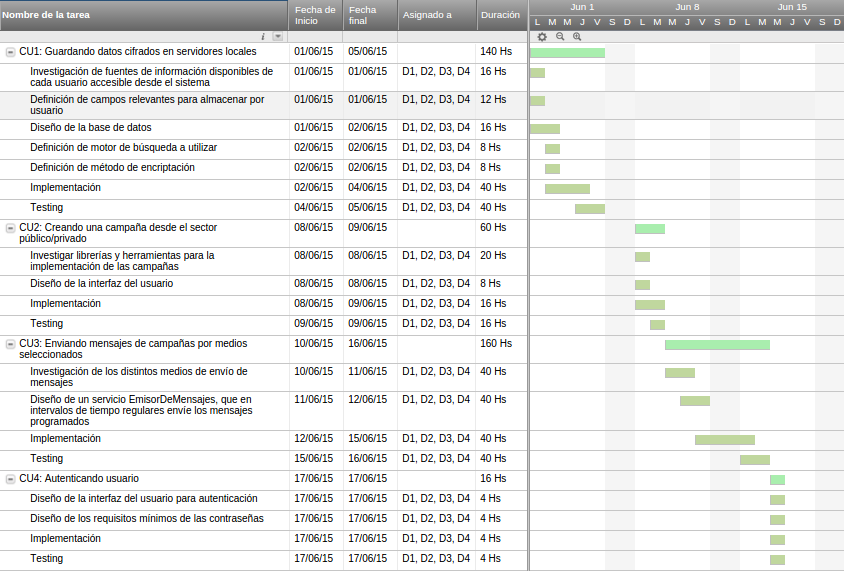
\includegraphics[width=20cm]{gantt.png}
  \caption{Diagrama de Gantt de la 1era iteración con la asignación de tiempo}
  \label{fig:gantt}
\end{figure}
\end{landscape}
\newpage

%%%%%%%%%%%%%%%%%%%%%%%%%%%%%%%%%%%%%%%%%%%%%%%%%%%%%%%%%%%%%%%%%%%%%%%%%%%%%%%
%% Análisis de riesgo                                                        %%
%%%%%%%%%%%%%%%%%%%%%%%%%%%%%%%%%%%%%%%%%%%%%%%%%%%%%%%%%%%%%%%%%%%%%%%%%%%%%%%

\section{Análisis de riesgos}

\riesgo{1}
    {Mantener la disponibilidad del servicio en la totalidad del país es importante. Sin embargo, se conoce que la disponibilidad del servicio puede tener dificultades en algunas zonas, como por ejemplo la patagonia.}
    {Alta}
    {Alto}
    {Alta}
    {Mantener un sistema que permita verificar la conexión de los distintos nodos que se encuentran en distintas regiones del país}
    {Al reportarse un fallo en la conexión, tercerizar la conexión a privados hasta que se arregle el problema}

\riesgo{2}
    {ArSat nos provee actualmente conexión y procesamiento en la región de Córdoba. Si se encuentra un problema en los nodos de ANSES, existirán problemas para procesar la información almacenada.}
    {Media}
    {Medio}
    {Medio}
    {Realizar backups de los nodos regionales con cierta frecuencia y almacenarlos de forma cifrada en una empresa tercerizada. Monitorear desde cada nodo el estado del resto de los nodos de las otras regiones mediante heartbeat.}
    {Notificar vía email al responsable técnico de un nodo al momento de detectarse su caída. Utilizar el backup cifrado en la empresa para lanzar una nueva instancia del nodo regional caído.}

\riesgo{3}
    {El modelo de abono que contabiliza los mensajes enviados está por migrar pronto a mejores servidores, por lo que se esperan algunas fallas de comunicación durante la transición.}
    {Alta}
    {Alto}
    {Alta}
    {Mantener un sistema de respaldo durante la migración del servicio para así poder asegurar la comunicación.}
    {Utilizar el sistema de respaldo para mantener la mayor correctitud posible los balances en el modelo de abonos a privados.}

\newpage

\section{Atributos de calidad}

Los atributos de calidad principales que debe respetar el sistema a realizar, en orden de prioridad, son los que siguen:

\begin{enumerate}
\item Disponibilidad
\item Performance
\item Seguridad
\item Certeza de Datos
\item Modificabilidad
\item Flexibilidad
\item Usabilidad
\end{enumerate}


Para describirlos, decidimos detallar escenarios correspondientes a cada uno de ellos.
Cada escenario está planteado en base al QAW y a los requerimientos o peticiones realizadas por los stakeholders en el enunciado.

\subsection{Disponibilidad}

\escenario{El sistema debe ser capaz de soportar fallas de los distintos enlaces de comunicación.}
    {Interna.}
    {Se produce una falla en la conexión.}
    {Operación degradada.}
    {Conexiones del sistema.}
    {Se cambia rápidamente a otro tipo de conexión.}
    {Se tarda a lo sumo 10 minutos en cambiar a otro enlace de comunicación.}

\escenario{Se quiere poder agregar nuevas campañas en todo momento.}
    {Interna.}
    {Un usuario desea agregar una campaña en el sistema.}
    {Operación normal.}
    {Sistema.}
    {El sistema permite crear una campaña en todo momoento.}
    {Cada intento de creación de campaña es exitoso bajo operación normal.}

\subsection{Modificabilidad}
\label{modificabilidad:atr1}
\escenario{Y pensar en ampliar los canales de comunicación además del SMS sumar Twitter, Whatsapp, Facebook Messenger, etc.}
    {Interna.}
    {Se desea extender el sistema.}
    {Operación normal.}
    {Sistema.}
    {El sistema es extensible a canales de comunicación en el menor tiempo posible.}
    {La extensión planteada no toma más de 8hs hombre modificando módulos relacionados.}


\subsection{Certeza de datos}
\escenario{Como el otorgamiento de información precisa en tiempo real es imposible (aún con el equipo necesario), se debe proveer datos estimados.}
    {Interna.}
    {Un usuario desea ver la evolución de una campaña.}
    {Operación normal.}
    {Sistema.}
    {Se presentan datos estimados de la campaña, lo más precisos posibles.}
    {Los datos presentados tienen una antiguedad de a lo sumo 10 minutos.}

\subsection{Seguridad}

\escenario{Quiere asegurar confidencialidad de todos los datos involucrados.}
    {Externa.}
    {Un individuo malintencionado intenta interferir los mensajes que se envían entre enlaces.}
    {Online.}
    {Sistema.}
    {Se utilizan cifrados para los mensajes los cuales tardarían un tiempo alto en romperse sin las claves correspondientes.}
    {Se tarda más de 10 mil años en realizar la decodificación sin claves.}

\escenario{Sólo personal autorizado y sus delegados en cada provincia tengan acceso a definir las campañas, y evolución.}
    {Externa.}
    {Un usuario sin privilegios intenta acceder a datos sobre campañas o definir una.}
    {Online.}
    {Sistema.}
    {Se utiliza un sistema de autenticación basado en usuarios y contraseñas. Se exigen contraseñas fuertes mediante restricciones de longitud mínima, combinación de caracteres alfanuméricos y especiales, etc.}
    {En las auditorías de seguridad sólo se logran adivinar las contraseñas de menos del 1\% de las cuentas de usuario.}

\escenario{Todos los datos que se manejarán son sensibles, y debe protegerse su acceso.}
    {Externa.}
    {Un individuo malintencionado intenta acceder a los datos guardados en las regiones o en el sistema de abono de datos.}
    {Online.}
    {Sistema.}
    {Se utilizan cifrados para los datos almacenados que tardarían un tiempo alto en decodificarse sin las claves correspondientes.}
    {Se tarda más de 10 mil años en realizar la decodificación sin claves.}

\subsection{Performance}

\escenario{Se debe poder monitorear el estado de las campañas de manera ágil. No se deben admitir demoras de ningún tipo.}
    {Externa.}
    {Un usuario desea ver el estado de una campaña.}
    {Operación normal.}
    {Sistema.}
    {Se visualiza el estado de la campaña.}
    {Se obtiene un reporte visual del estado de la campaña en menos de 10 segundos.}

\escenario{Se quiere que distintas empresas puedan tener acceso rápidamente a los datos de evaluación para mejorar los perfiles de marketing.}
    {Interna.}
    {Una empresa desea acceder a los datos de evaluación.}
    {Operación normal.}
    {Sistema.}
    {Se reportan los datos de evaluación de las campañas solicitadas.}
    {Se obtiene un reporte del estado de evaluación de las campañas solicitadas en menos de 10 segundos.}

\subsection{Usabilidad}

\escenario{Se quiere que el sistema sea fácil de usar para todos aquellos interesados en promover campañas de todo tipo.}
    {Interna.}
    {Un usuario desea poder utilizar fácilmente el sistema para crear campañas.}
    {Operación normal.}
    {Sistema.}
    {Los usuarios pueden utilizar fácilmente el sistema.}
    {Los usuarios tardan menos de 30 minutos en aprender a crear campañas en el sistema.}

\newpage

\section{Arquitectura BigTiza}

\subsection{Diagrama de componentes y conectores}
En lo que sigue, presentamos la arquitectura del trabajo con vista de Componentes y Conectores. Para la realización de la misma, utilizamos conectores creados específicamente para nuestras necesidades. Éstos son:

\begin{figure}[h!]
  \diagramadeancho{12cm}{./diagramas/referenciadeconectores.pdf}
  \caption{Referencia de los conectores creados.}
\end{figure}

\begin{itemize}
  \item \textbf{Conector encriptado asíncrono:} conector asíncrono de la cátedra con cifrado.
  \item \textbf{Conector selector asíncrono:} funciona como un proxy, redirige los datos por el sistema de ArSat o por el sistema de abono de datos hasta su destino. Prioriza el sistema de ArSat, si este no está disponible utiliza el sistema de abono de datos. Guarda la cantidad de datos que se envían por el sistema de abono de datos para llevar auditoría de lo utilizado. Los datos siempre viajan cifrados. Se encuentra definido a posteriori.
  \item \textbf{Conector asíncrono:} conector clásico de la cátedra.
  \item \textbf{Conector encriptado client/server:} conector client/server de la cátedra con cifrado.
  \item \textbf{Conector selector client/server:} conector selector definido anteriormente con capacidad client/server.
  \item \textbf{Conector síncrono:} conector clásico de la cátedra.
  \item \textbf{Conector repositorio encriptado:} conector clásico de la cátedra con cifrado.
  \item \textbf{Conector client/server:} conector clásico de la cátedra.

\end{itemize}

\newpage

\subsection{Diagrama de componentes y conectores}


\subsubsection{Nodo regional}

\diagramadeancho{14cm}{./diagramas/nodoregional.pdf}
\newpage


\subsubsection{Actuador web}

\diagrama{./diagramas/actuadorweb.pdf}
\newpage


\subsubsection{Emisor de mensajes}

\diagrama{./diagramas/emisordemensajes.pdf}
\newpage


\subsubsection{Receptor de mensajes}

\diagramadeancho{12cm}{./diagramas/receptordemensajes.pdf}
\newpage


\subsubsection{Conector selector (proxy)}

\diagrama{./diagramas/conectorselector.pdf}
\newpage


\subsection{Justificación de la arquitectura}

Para la realización de la arquitectura correspondiente al Sistema BigTiza se tuvieron en cuenta, principalmente, los atributos de calidad descritos anteriormente. La vista construída corresponde a la de \textit{Componentes y Conectores}. En lo que sigue, explicamos la arquitectura realizada.

En primer lugar, decidimos representar la interfaz a la que accede un usuario con un \textit{Servidor web}. Éste se encarga únicamente de servir la interfaz de usuario, y delega al \textit{Actuador web} la realización de cualquier operación que solicite el usuario por medio de la interfaz web.

Utilizamos un repositorio de campañas para el almacenamiento cifrado de los datos y otro para el almacenamiento de campañas (los mensajes de cada una de éstas).

Utilizamos un repositorio de usuarios, donde se guardan los usuarios y las contraseñas de los mismos.

El repositorio de grupos de personas almacenan los números de las personas por su categoría (si son fumadores, si son deportistas, etc.).



El \textit{Conector selector} (cumpliendo el rol de un proxy) verifica si el sistema de Arsat está caído, en cuyo caso elige la opción de utilizar el sistema de abono para la comunicación entre nodos regionales.

El \textit{Actuador} recibe las peticiones web y las atiende.



\subsubsection{Nodo regional}

\begin{itemize}

  \item El servidor web sirve la interfaz y atiende pedidos de operaciones, que son delegadas al actuador web.
  \item El actuador web ...

\end{itemize}


\subsubsection{Receptor de mensajes}

A grandes razgos, el componente \textit{Receptor de mensajes} tiene la responsabilidad de recibir los mensajes entrantes correspondientes a las respuestas de las preguntas realizadas para la evaluación de las campañas.

El componente cuenta con la siguiente estructura:

\begin{itemize}
  \item Un bus publish/subscribe con tres componentes de recepción de mensajes vía SMS, Whatsapp y email que se comunican con los servicios externos correspondientes y publican los mensajes en el bus a medida que llegan. La motivación del bus publish/subscribe también es permitir la facilidad de cambio a la hora de agregar nuevos canales de envío y recepción de mensajes, cumpliendo con el atributo de modificabilidad mencionado en \ref{modificabilidad:atr1}.

  \item Un componente \textit{Director de mensajes} el cual se subscribe a al bus descripto para recibir los mensajes o respuestas recibidas de distintos medios. Este componente procesa las respuestas para que el \textit{Actualizador de datos de evaluación de campañas} pueda consumirlas, pudiendo posteriormente realizar las actualizaciónes correspondientes.

\end{itemize}

\subsubsection{Emisor de mensajes}

El componente \textit{Emisor de mensajes} cuenta con los siguientes componentes:

\begin{itemize}
  \item Un \textit{Notificador de mensajes a enviar}, que consulta periódicamente al \textit{Repositorio de campañas} auxiliado del \textit{System timer} para decidir los mensajes que requieren ser enviados, y decide los destinatarios de los mismos consultando al \textit{Repositorio de grupos de personas}. Una vez conocidos los mensajes y los destinatarios, se publican los mismos en el bus publish/subscribe anterior.

  \item Un bus publish/subscribe, al que subscriben tres componentes: \textit{Emisor de mensajes via email}, \textit{Emisor de mensajes via Whatsapp} y \textit{Emisor de mensajes via SMS}. Éstos toman los mensajes que les corresponden del bus para efectuar el envío de los mensajes mediante los distintos servicios externos. Se utiliza un bus publish/subscribe para permitir fácilmente y con impacto mímimo la incorporación de nuevos emisores para nuevos canales de envío en el futuro, satisfaciendo el atributo de modificabilidad planteado anteriormente en \ref{modificabilidad:atr1}.
\end{itemize}

\subsubsection{Actuador web}

\begin{itemize}
\item El Receptor de mensajes web se encarga de aceptar los mensajes provenientes de la interfaz web. El mismo cataloga a qué componente le corresponde atender el mensaje recibido.
\item El Administrador de grupos de personas se encarga de seleccionar a las personas afectadas por la petición recibida. El mismo busca los usuarios necesarios en el Repositorio de grupos de personas, que se encuentran previamente fraccionados por distintos criterios (por ejemplo: fumador, no fumador).
\item El Receptor de mensajes heartbeat se encarga de recibir las señales heartbeat de los distintos nodos pertenecientes al sistema. En el caso en el que alguno de ellos no fuera recibido, se envía la notificación al Servicio mail. Por lo tanto, el Receptor de mensajes es también el encargado de verificar que todos los nodos hayan enviado su señal heartbeat.
\item El Emisor de señales heartbeat envía cada cierta frecuencia un ``latido'' que recibirán los receptores de señales heartbeat del resto de los nodos.
\item El Receptor de datos de evaluación manual recibe resultados medidos manualmente por los usuarios para guardarlos en el Actualizador de datos de evaluación de campañas. Por ejemplo, si un usuario desea almacenar en el sistema la cantidad de asistencias a una carrera o cantidad de aprobados en un examen, lo debe ingresar manualmente en el sistema.
\item El Administrador de campañas recibe los mensajes del Receptor de mensajes web que corresponden a la gerencia de campañas. Entre las peticiones posibles, se encuentran la creación, modificación y supresión de campañas como también la provisión de resultados de las mismas. Dicha información se encuentra almacenada en los Repositorios correspondientes a las campañas. Por otro lado, el Administrador se comunica con otros nodos regionales para proveerles información sobre las campañas en caso de que lo requieran.
\item El Reportador de resultado de campaña responde los petitorios correspondientes a los resultados que se generan en base al Repositorio de datos de campañas (que conserva la totalidad de mensajes recibidos y los datos que puedan servir para la evaluación de los resultados). Dichos resultados son valores que se actualizan en el Caché de evaluación de campañas.
\end{itemize}

\subsubsection{Conector selector}

El conector está compuesto por un \textit{proxy de conexión} el cual se encarga de transmitir la información que recive del \textit{emisor de mensajes} y asegura la disponibilidad de la conexión. Para esto, verifica si el sistema de Arsat esta caído, en cuyo caso, le envía la información al \textit{componente receptor} a traves del \textit{sistema de abono privado}. Por otro lado, se encarga de actualizar en el \textit{repositorio de uso de datos}, la cantidad de información que fué enviada a traves del \textit{sistema de abono privado}. 

Toda la información que se envía mediante este conector es cifrada para garantizar que la conexíón es segura y que ninguna persona la puede robar y$/$o modificar.

\newpage


%%%%%%%%%%%%%%%%%%%%%%%%%%%%%%%%%%%%%%%%%%%%%%%%%%%%%%%%%%%%%%%%%%%%%%%%%%%%%%%%
% Arquitectura del TP 1                                                        %
%%%%%%%%%%%%%%%%%%%%%%%%%%%%%%%%%%%%%%%%%%%%%%%%%%%%%%%%%%%%%%%%%%%%%%%%%%%%%%%%


\section{Arquitectura del TP 1}

Para la arquitectura del TP 1, nos basamos en el diagrama de clases realizado considerando las decisiones tomadas a lo largo de la elaboración del mismo.

\begin{itemize}
\item El \textit{Servidor web} representa a la interfaz que se le muestra al usuario cuando desea ingresar al sistema.
\item El \textit{Receptor de peticiones web} se encarga del manejo de los pedidos realizados por los usuarios. Éstas pueden incluir información sobre las mediciones de eficacia, sobre el estado de las campañas, agregado o supresión de mensajes, etc.
\item El \textit{Autenticador} verifica el usuario y la contraseña ingresados por el usuario para otorgarle los permisos que le corresponden.
\item El \textit{Repositorio de credenciales} envía la información al \textit{Autenticador}, quien almacena la información de los directivos y maestros.
\item El \textit{Repositorio de mensajes} almacena los mensajes de las campañas. Funciona como repositorio (cuando un mensaje debe ser enviado al emisor de mensajes) y como blackboard (cuando un usuario agrega un nuevo mensaje).
\item El \textit{Repositorio de eventos} tiene guardados los eventos de las campañas y tiene el mismo rol que el repositorio de mensajes.
\item El \textit{Emisor de mensajes} es el encargado de transmitir los mensajes en tiempo y hora junto con los destinatarios de los mismos al \textit{Servicio de SMS} para que éste los envíe.
\item Para la realización de esto último, el \textit{Repositorio de alumnos} (que incluye a los padres de los mismos) le provee los datos necesarios al \textit{Emisor de mensajes} para que se les envíe el mensaje a los alumnos correspondientes.
\end{itemize}

El diagrama resultante es el siguiente:

\diagrama{./diagramas/arquitecturaTP1.png}

\newpage


%%%%%%%%%%%%%%%%%%%%%%%%%%%%%%%%%%%%%%%%%%%%%%%%%%%%%%%%%%%%%%%%%%%%%%%%%%%%%%%%
% Comparación entre arquitecturas de TPs 1 y 2                                 %
%%%%%%%%%%%%%%%%%%%%%%%%%%%%%%%%%%%%%%%%%%%%%%%%%%%%%%%%%%%%%%%%%%%%%%%%%%%%%%%%


\section{Comparación entre arquitecturas de TPs 1 y 2}

Como primer diferencia entre las arquitecturas del TP 1 y TP 2, podemos observar un importante incremento en la complejidad de las mismas al pasar de un sistema de un único servidor en una escuela a uno de gran escala capaz de soportar diferentes tipos de mensajes y distribuido en diferentes lugares del país.

A grandes rasgos, la apariencia de ambas arquitecturas es similar; hay repositorios de usuarios y mensajes, un servidor web para acceder al sistema y servicios de mensajes que se encargan del envío. Sin embargo, el sistema del TP2 se adapta a grandes escalas y amplias tecnologías que obligan a considerar una mayor cantidad de servicios, control del resto de los sistemas, múltiples conexiones y backups de los sistemas.
\begin{comment}
En primer lugar observamos que al tener mensajes de directos sensores en la tierra no necesitábamos drones para tomar fotos ni componentes para analizar imágenes,
la información sobre el suelo era accesible directamente.

De un modo similar en la comunicación con la interfaz meteorológica evitábamos tener que localizar el lugar de origen de los datos, y nos ahorramos
los componentes específicos para analizar los datos. 

Por otro lado, al haber menor necesidad de guardar información a lo largo del tiempo, hacían falta menos repositorios distribuidos a lo largo de la arquitectura.
El único repositorio de la arquitectura actual que viene de la arquitectura del TP anterior es el de Plan(es) Maestro(s), un concepto que sobrevive todo cambio de
arquitecturas por su importancia en el dominio.
Muchos de los repositorios nuevos que se agregaron tienen que ver con el gran flujo de datos y eventos y la imposibilidad de responder a todos ellos en tiempo real,
algo que en el TP1 no ocurría.

En general vemos que la sucesión de colaboraciones desde la llegada de nueva información hasta el accionar (o no) de los actuadores 
era mucho más simple y corta en el TP1 que en el 2do, presentando componentes con responsabilidades más generales, como los ``Supervisores'' que combina responsabilidades
de que en el TP2 aparecen distribuidas entre la comunicación con los sensores, el analizador de los datos, almacenador, controlador de estadios, planificador, etc.

Sin embargo, si bien las diferencias son variadas y profundas, observamos cierta similitud general entre los diagramas. Algo que podríamos llamar la ``esencia'' de la 
arquitectura permaneció intacto de un TP a otro (aunque casi imposible de visualizar al ojo no entrenado en el dominio del problema). Dicho en términos de la materia,
ambas arquitecturas presentan un estilo similar: existen sensores, el sistema les pide información a esos sensores, la procesa y en función del resultado y de 
lógicas preestablecidas que consulta a partir de repositorios toma decisiones que envía a un conjunto de actuadores que intervienen en el medio de la(s) planta(s).
\end{comment}

\newpage


%%%%%%%%%%%%%%%%%%%%%%%%%%%%%%%%%%%%%%%%%%%%%%%%%%%%%%%%%%%%%%%%%%%%%%%%%%%%%%%%
% Conclusiones                                                                 %
%%%%%%%%%%%%%%%%%%%%%%%%%%%%%%%%%%%%%%%%%%%%%%%%%%%%%%%%%%%%%%%%%%%%%%%%%%%%%%%%


\section{Conclusiones}

Desde el punto de vista del desarrollo tenemos pocas herramientas para comparar los métodos usados a lo largo de la materia (Scrum y UP),
dado que trabajando con Scrum realizamos una única iteración y trabajando con UP ni siquiera llegamos a desarrollar nada efectivamente.
Además, como cada método lo aplicamos a proyectos de tamaños distintos, la comparación que hagamos estará sesgada por cosas propias de la
complejidad de los problemas que quizás no forman parte de la metodología en sí, entorpeciendo nuestra capacidad de diferenciarlas únicamente
por sus características.

Sin embargo, sí pudimos comparar las etapas iniciales de ambas metodologías, viendo claramente una diferencia entre realizar una planificación
y un diseño antes de comenzar a programar; y empezar a programar sin planificación previa e ir diseñando a medida que se desarrolla. Si bien
en el primer TP consideramos que nuestra aplicación de Scrum era imperfecta pues estábamos acostumbrados a diseñar por adelantado,
en este segundo TP descubrimos que se puede planificar a un nivel más profundo del que conocíamos.

Desde un punto de vista subjetivo, podemos resaltar de UP la priorización de los atributos de calidad como ``drivers'' de las decisiones arquitectónicas,
entendiendo que con Scrum se podrían perder de vista en pos de resolver cuestiones funcionales, y que modificar una aplicación ya construida para que
satisfaga cierto atributo de calidad no contemplado previamente es mucho más costoso que diseñarla teniéndolo en cuenta desde un principio.

Sin embargo, preferimos Scrum a la hora de organizar los tiempos y responsabilidades del proyecto. Como ya dijimos no tuvimos la oportunidad de
experimentarlo nosotros mismos, pero consideramos que, por ejemplo, un error en la estimación de esfuerzo en Scrum tiene consecuencias mínimas
en comparación con las que tendría el mismo error (de estimación de horas/hombre) en UP: en Scrum como mucho una historia quedará afuera de una iteración y
tendrá que ser subdividida más adelante, mientras que en UP puede producir un efecto dominó que afecta todas las iteraciones posteriores
(porque ya se planificaron previamente) y eventualmente postergar todo el proyecto en caso de que la tarea sea crítica.

Entendemos, de todos modos, que combinar las características que destacamos de cada una de las metodologías es no-trivial. Afortunadamente, proponer una metodología
superadora excede el scope de este trabajo práctico.

A la hora de la comparación entre ``programming in the small'' y ``programming in the large'' podemos mencionar la diferencia entre las vistas más usadas: a la hora del 
diseño OO utilizamos tanto diagramas de clases (estático) como de objetos (dinámico) mientras que en la arquitectura se le da más importancia a la vista de
componentes y conectores (dinámica). Creemos que esto tiene que ver con que la arquitectura a gran escala se puede apreciar de manera más simple cuando vemos
cómo estarán los componentes ``en funcionamiento''.

Otra característica distintiva, aunque quizás sea un sesgo de parte de las metodologías usadas, es que la programación a pequeña escala está más orientada
a cumplir con atributos funcionales, mientras en que la programación a gran escala hay que darle mucha más relevancia a cuestiones no funcionales. Esto podría explicarse
si pensamos que en geneneral los productos más grandes son los que tienen más riesgos asociados relacionados con escalabilidad, seguridad, performance, etc.

Desde el punto de vista específico de la realización del trabajo, encontramos dificultades para diferenciar el análisis de riesgos de los atributos de calidad.
En mayor o menor medida, descubrimos que la mayoría de los atributos de calidad tienen algún riesgo relacionado (y viceversa), por lo que por momentos nos 
parecía redundante realizar ambos análisis. Quizás la diferencia se nota mejor en un proyecto real con stakeholders reales en el cual el análisis de riesgos
precede temporalmente a la documentación de atributos de calidad, pero de todos modos encontramos muchos puntos comunes a ambos análisis.

\end{document}
